\newpage

\section{Remerciements}\label{remerciements}

\bigskip

Je tiens à remercier Benjamin Tierny, Robin Komiwes et Julien Vanden
Torren de m'avoir acceuilli chez Dernier cri pour mon stage.

\bigskip

Je remercie également mon suiveur Harry Claisse pour son aide et son
accompagnement, ainsi que les enseignants de l'Université technologique
de Compiègne.

\bigskip

Merci également à toute l'équipe de Dernier cri pour avoir rendu mon
stage si enrichissant et agréable.

\newpage

\section{Résumé et abstract}\label{ruxe9sumuxe9-et-abstract}

\bigskip

\subsection{Résumé}\label{ruxe9sumuxe9}

\newpage

\subsection{Abstract}\label{abstract}

\newpage

\section{Introduction}\label{introduction}

\bigskip

Dans le cadre de mon TN09 à l'Université technologique de Compiègne,
j'ai effectué un stage de six mois chez Dernier cri.

\bigskip

Dernier Cri est une Start-Up crée en 2011 spécialisé dans l'innovation
numérique. L'équipe est en charge du développement, du déploiement et de
la maintenance d'applications pour le compte de plusieurs clients.

\bigskip

Ma mission à été d'intégrer l'équipe de developpement pour aider dans la
création de plusieurs applications web.

\bigskip

J'ai pus lors de ce stage intégrer une équipe dynamique et pro-active.
J'ai notamment pus prendre part à de nombreuses présentations internes
sur différentes technologies, à l'écriture d'article de blog. J'ai
également pus participer activement à la relation cliente lors de mes
projets.

\newpage

\section{Dernier cri}\label{dernier-cri}

\bigskip

\subsection{Histoire}\label{histoire}

\bigskip

En 2011 Robin Komiwes et Benjamin Tierny créent Nectify dans le but de
développer \textbf{Fresc}, un outil de partage d'avis sur des visuels.
Bien que cet outil connait un succés certain avec aujourd'hui plus de
300 sociétés utilisant Fresc à travers des milliers de projets, la
rentabilité du projet n'est pas suffisante.

\bigskip

Nectify choisi alors de compléter ses revenus par de la prestation de
services centrée sur l'innovation.

\bigskip

Début 2014, la majeure partie du chiffre d'affaire de Nectify était dû
aux activités de prestations de services, Fresc ne représentant qu'une
part marginale.

\bigskip

Devenant donc une agence spécialisée dans l'innovation digitale, Nectify
choisi de changer de créé sa propre image, distincte de Fresc. C'est
dans se mouvement que la société est devenu \textbf{Dernier cri}.

\bigskip

Aujourd'hui \textbf{Dernier cri} est une agence web

(Dernier Cri met un point d'honneur à proposer à ses clients une
solution complète adaptée à un problème spécifique. De la conception à
la réalisation, l'entreprise accompagne ses clients de A à Z pour
aboutir à un produit au plus proche des besoins de ceux-ci. Cela permet
aux développeurs d'opérer dans différents domaines d'activités et
d'avoir une vue globale du développement de produit.)

\bigskip

\begin{figure}
\centering
\includegraphics{logo_DC}
\caption{logo}
\end{figure}

\newpage

\subsection{Secteur d'activité}\label{secteur-dactivituxe9}

\bigskip

\subsection{Organisation}\label{organisation}

\bigskip

L'entreprise est constitué de 16 employés. Le CEO de l'entreprise est
Benjamin Tierny, co-fondateur de Dernier cri, tandis que Robin Komiwes
est CTO.

\bigskip

Le troisième associé, Julien Vanden Torren, est Account Manager. C'est à
dire le lien entre l'entreprise et les clients.

\bigskip

L'entreprise est également constitué d'une chef de projet, Laetitia
Cocusse, qui s'occupe de superviser la pluspars des projet.

\bigskip

L'équipe de développeur est constitué notament d'un devops, c'est à dire
possédant à la fois les compétences d'un développeur et d'un ingénieur
système (Jean-Serge Monbailly), d'un Data Scientist (Antonin Carette)
qui travaille sur les projet de big data.

\bigskip

La plupars des développeurs travails sur plusieurs projets en même
temps, selon les besoins de l'entreprise et les compétences de chacun.
Des équipes de 2/3 developpeurs sont créé, mélangeant les compétences
front et back, de developpement et de systeme.

\bigskip

\begin{figure}
\centering
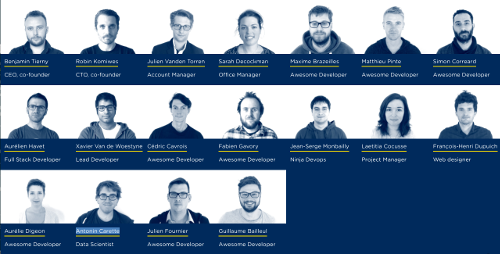
\includegraphics{team.png}
\caption{image}
\end{figure}

\subsubsection{Github et code review}\label{github-et-code-review}

\bigskip

L'entreprise utilise principalement la plateforme Github comme service
web d'hébergement et donc le logiciel de gestion de versions Git. Github
permet au developpeur de travailler à plusieurs sur le même projet, de
résoudre rapidement des conflits dus à la modification d'un même
document pars plusieurs personne, de gérer différente version du projet
etc\ldots{}

\bigskip

Une nouvelle version de Githib propose une section \textbf{Projet}
permttant de gérer les \textbf{issues}, c'est à dire les taches. Cette
section permet de notamment de séparer les taches en plusieur colonnes,
par exemple : \emph{A faire}, \emph{En cours}, \emph{Terminé}. Il est
aussi possible d'attribuer les taches à un contributeur, ou encore de
leur attribuer des labels tel que \emph{Urgent}, \emph{Bug} ou encore
une estimation de temps quand à la réalisation de la tache.

\bigskip

Dernier cri utilisait jusque la un outil similaire. Il a été décidé
d'utiliser la section \textbf{Projet} de Github pour les nouveaux
projets, notamment ceux sur lesquels j'ai étais affecté.

\bigskip

Github offre aussi un outils de \emph{Code Review}, c'est à dire de
relecture du code avant son incoration au projet. Dernier cri utilise ce
systéme pour garantir une certaine qualité du code ainsi qu'un style
d'écriture homogéne. C'est également l'occasion pour les développeurs

\bigskip

Dernier cri à mis en place un processus de vérification de la qualités
du code et d'entraide. Chaque developpeur, une fois une tache terminé,
propose une \emph{Pull request}, c'est à dire demande à fussionner sa
version du projet, modifié pour résoudre la tache, avec la version
principal, stable. Il demande ensuite à ses collégues ayant des
compétences dans le langage utilisé de relire et de commenter cette
\emph{Pull request}.

\bigskip

Ce processus permet non seulement de garantir la qualité du code mais
permet aussi de proposer des solution, des syntaxes alternatives, que
peut être le developpeur ne connaissait pas. Bien souvent c'est aussi
l'occassion de débatre sur le bien fondé d'habitudes, ou de conventions.

\bigskip

\subsubsection{Talk interne}\label{talk-interne}

\bigskip

Dans l'optique du partage du savoir dans l'entreprise, les employés sont
invités à faire des présentation en interne. Les présentation peuvent
autant porter sur des langages de programmation, des nouvelles
technologies, de la gestion de projet \ldots{}

\bigskip

Les talks techniques permettent aux membres d'une équipe de partager
entre eux des points de vue, des techniques/conseils. Cela permet
d'interresser les autres sur certain sujets. Pour la personne organisant
la conférences c'est aussi une occasion de travailler sur ces
compétences de synthése etc\ldots{}

\bigskip

Durant mon stage j'ai eu l'occasion d'assister à des présentation sur
React, Docker, Rust, MJML

\bigskip

Ces présentations sont publiées sur la
\href{https://www.youtube.com/channel/UCDfdBlzldhg_PEu3xZTPsHg}{chaîne
youtube Dernier cri}

\bigskip

-\textgreater{} Voir article de Xavier pour completer

\subsubsection{Article de blog}\label{article-de-blog}

\bigskip

Dernier cri posséde également un
\href{http://derniercri.io/tech-blog}{blog technique} alimenté par les
developpeurs de l'équipe.

\bigskip

Les objectifs sont notablement les même que pour les présentations
interne. Mais cela permet aussi à Dernier cri de rayonner et montrer ses
compétences techniques et son esprit d'anlayse. Les commentaires
permettent aussi d'échanger avec la communauté web.

\newpage

\section{Cadre du stage}\label{cadre-du-stage}

\bigskip

-\textgreater{} Relation clients -\textgreater{} Mise en production

Durant mon stage j'ai pus participer au développement de deux
applications. Ces deux projets s'appuyé sur du React, une bibliothèque
JavaScript libre développée par Facebook depuis 2013. N'ayant jamais
utilisé cette bibliothéque, j'ai donc du tout d'abord me former.

\bigskip

Le premier projet auquel j'ai participé se nomme Photolix. C'est un site
internet de développement de photos, avec pour objectifs de toucher un
public \ldots{}. et de limiter au maximum le temps d'attente du client
en envoyant les photos au serveur dès leur sélection.

\bigskip

Le second projet est FinFrog, un site proposant des prêts financés par
des particuliers. Ce projet était déjà assez avancé à mon arrivé. Le
client possédait un site en ligne, mais souhaité changer l'apparence et
ajouter des fonctionnalités, ce pourquoi il a fait appel à Dernier cri.

\subsection{Formation}\label{formation}

\bigskip

Lors de mon arrivée chez Dernier cri, j'ai eu l'occasion de me former
sur Javascript ES6, React ainsi que Redux, car l'entreprise prévoyé de
me mettre sur des projets utilisant ces technologie.

\bigskip

Ces trois technologie étant \ldots{} (ca m'intéresse et en plus c'est
hype)

\bigskip

Ma formation c'est faite à partir du site
\href{https://www.codeschool.com/}{Code school}, disposant de cours en
vidéos ainsi que d'exercices intéractifs.

\bigskip

\subsubsection{Javascript ES6}\label{javascript-es6}

\bigskip

Le Javascript est un langage de programmation de scripts incourtounable
du web. Si à sa création il servait principalement à la réalisation
d'animation, il est aujourd'hui au centre des applications. Le javacript
sert maintenant à controler presque la totalité de l'application web.
Cependant, ce langage n'étant pas était prévu pour une telle compléxité,
il en résulte une syntaxe complexe et lourde. C'est dans ce contexte
qu'un mise à jour du langage c'est imposé.

\bigskip

ES6 (ECMAScript Edition 6 ou encore ES2015) a été publiée en juin 2015.
Il ajoute un ensemble de normes a celles déja présente pour apporter de
nouvelle fonctionnalités qui permettent d'alléger le code, de le
structurer, et de le rendre notamment plus maintenables, tout en restant
compatibles avec le code existant.

\bigskip

ES6 n'est pas encore totalement supporté par les navigateurs, il est
donc utilise d'utiliser un transcompilateur vers ES5, comme Babel.js.

\bigskip

L'apprentissage de ES6 a était primordiale pour mon stage : les
nouvelles normes rende vraiment le code plus facile à lire et à écrire.
J'ai eu l'occasion durant mon stage de travailler sur un projet
JavaScript n'utilisant pas ES6 et j'ai eu de grande difficultés à me
passer des facilité d'écritures.

\bigskip

\subsubsection{React}\label{react}

\bigskip

Developpé depuis 2013 par Facebook, React est une bibliothèque
JavaScript déclarative, efficace et flexible pour la création
d'interfaces utilisateur. Cette bibliothéque c'est démarqué notamment
par ses performances.

\bigskip

Elle est aujourd'hui utilisé par de nombreuses entreprises tel que
Netflix, Yahoo, Airbnb ou encore Sony.

\bigskip

Une des particulariés de React est de découper l'application en
composants, dépendant d'un état. Lors du changement de l'état d'un
composant, React génére les changements en HTML pour les répercutés sur
la page. Grace à l'utilisation d'un DOM virtuel, c'est à dire d'une
représentation de la vue, React fait le minimum de modification
possible, ce qui explique ces performances.

\bigskip

Cette bibliothéque est aujourd'hui en expensions. Elle a un succés
certain auprès de la communautés des developpeurs web, et de nombreux
outils se developpe autours. C'est donc un avantage certain d'avoir pu
apprendre React lors de mon stage, puis d'avoir mis en pratique ces
connaissances lors des deux projets que j'ai effectués.

\bigskip

\subsubsection{Redux}\label{redux}

React, même s'il n'impose pas de bibliothèque pour les data et la
communication des modules, offre une approche nommée flux très
intéressante et vous offrant des clés pour concevoir une app avec en
tête les paradigmes pensés pour React.

En plus de React, Facebook à fournit une architecture appelé
\textbf{Flux}. Cette architecture promet un flot unilatéral des données
pour que le developpeur puisse facilement suivre le trajet de des
données d'un événement et ses conséquences. Ce pattern s'appuie sur
trois éléments: les dispatcher, les stores et les vues (Les components
React).

\textbf{Redux} est une des implémentation de \textbf{Flux} les plus
populaire, créée en Mai 2015 par Dan Abramov. Bien que reprenant les
concepts de Flux, Redux les simplifie en utilisant des concepts liés à
la programmation fonctionnelle.

On peut résumer Redux par ses 3 grands principes : * L'état de toute
l'application est stocké dans un unique \textbf{store}. * L'état est en
\textbf{lecture seule}. La seule façon de le modifier est l'utilisation
d'\textbf{action} décrivant la modification voulu. * Les modifications
sont faites avec des \textbf{fonctions pures}, c'est à dire une fonction
qui prend l'état précédent et retourne un nouvel objet, le nouvel état.

Même si la mise en place de \textbf{Redux} peut sembler dans un premier
temps laborieuse, cette architecture à l'avantage d'offrir une bonne
lisibilité quand au changement d'état, ce qui est utilise dans les
grandes applications.

\subsection{Gestion de projet}\label{gestion-de-projet}

Le processus de developpement chez Dernier cri se passe comme suit :
notre chef de projet, Laetitia Cocusse, discute avec le client pour
comprendre ses besoins et ses attentes. Selon les besoins, elle organise
une réunion avec le(s) developpeur(s) et le client pour clarifier
certain point ou pour discuter des différents approches du problémes
possible. C'est l'occasion pour le developpeur de proposer des
solutions, peut être un peut différentes de celle imaginait par le
client, ou encore de dire son avis sur les prochaines taches.

\bigskip

Ensuite les taches sont estimées en temps par un developpeur. Cette
estimation devra ensuite étre validée par le client.

\bigskip

Une fois la tache validée, une \emph{issue} est créé dans Github avec
une description, l'estimation et le developpeur à qui est attribué la
tache.

\bigskip

Selon les priorités, le developpeur choisi ou non l'ordre des taches.
Pour proteger le projet actuel, stable, des nouvelles modification tant
que celle-ci ne sont pas tester, le developpeur crée une \emph{branche}
dans Github, c'est à dire une copie du projet qui évoluera
indépendamment de la branche principale. C'est sur cette branche que
seront faites les modifications destinées a implémenter la nouvelle
fonctionnalité.

\bigskip

Une fois le developmment de la fonctionnalité fait, la nouvelle version
du site est déployé en \emph{staging}, c'est à dire une version en ligne
du site, qui à le même environnement que la production, mais avec des
fausses données. Ce site sert à tester les nouvelles fonctionnalités
avant de les pousser sur la production.

\bigskip

Laetitia fait une \emph{recette}, c'est à dire vérifie que la version de
staging remplie bien le besoin exprimé par le client, et que la nouvelle
fonctionnalité n'a pas cassé autre chose. En cas de problème, le
developpeur reviens sur la tache jusqu'a ce que tout soit réglé.

\bigskip

Une fois un lot de taches effectuées, il est décidé en accord avec le
client de poussé les modifications sur la production. Il faut alors
vérifier que la \emph{mise en prodcution} c'est bien passé : que le site
fonctionne toujours et que les nouvelles fonctionnalités sont bien en
place.

\bigskip

\subsection{Photolix}\label{photolix}

\subsubsection{Présentation du projet}\label{pruxe9sentation-du-projet}

\bigskip

Dès mon arrivée dans l'entreprise j'ai été assigné a la réalisation
d'une application de developpement photo. Le client posséde un studio de
developpement photo sur Lille, et souhaité proposé à ses clients un site
simple et efficace.

\bigskip

Le principal objectif de ce projet était d'uploader les photos au fur et
à mesure de leur selection, pour ainsi éviter le temps d'attente du
client à la fin de la saisie de ces informations.

\bigskip

Lors de mon arrivée sur le projet, un développeur de dernier cri avait
déja posé des bases. Les fonctions de recadrage et de compression de la
photo étaot notamment déjà écrite.

\bigskip

\subsubsection{Objectifs}\label{objectifs}

\subsubsection{Déroulement}\label{duxe9roulement}

\subsubsection{Difficultés}\label{difficultuxe9s}

\subsubsection{Conclusion}\label{conclusion}

\subsection{Finfrog}\label{finfrog}

\subsubsection{Présentation du
projet}\label{pruxe9sentation-du-projet-1}

\subsubsection{Nouveaux outils}\label{nouveaux-outils}

\subsubsection{Organisation}\label{organisation-1}

\subsubsection{Difficultés}\label{difficultuxe9s-1}

\section{La vie Lilloise}\label{la-vie-lilloise}

\subsection{Take Off Conference}\label{take-off-conference}

\bigskip

Dernier cri m'a donné l'occasion durant mon stage d'assister à la
\href{http://takeoffconf.com/2016}{\textbf{Take Off Conference}} les 20
et 21 octobre 2016. Cette évenement à lieu depuis plusieurs années à
EuraTechnologies, le Pôle d'excellence économique dédié aux Technologies
de l'Information et de la Communication de la métropole lilloise.

\bigskip

Historiquement, ce sont les fondateurs de Dernier cri qui ont créé la
\textbf{Take Off Conference}, avec Florian Le Goff. Aujourd'hui ce sont
d'autre acteur de la communauté web de Lille qui ont pris le relais pour
proposer une nouvelle édition.

\bigskip

La \textbf{Take Off Conference} est un cycle de conférences anglophones.
L'événement dure 2 jours, et accueille des conférenciers du monde
entier. Bien qu'elle reste avant tout une conférence pour les
développeurs Web, elle reste accessible pour les développeurs en
général.

\bigskip

Dernier cri m'a permis de participer à cette conférence avec l'un de mes
collègues. Ce fut une véritable chance pour moi de rencontrer et
échanger avec des conférenciers du monde entier. Les conférences étaient
très intéréssantex et inspirantes, sur des sujets très varié allant de
\ldots{}.

\bigskip

Des évènements ont également été organisé le soir pour permettre au
participant et au conférenciers d'échanger dans un cadre puis détendue.

\bigskip

Ce fut une excellente occasion de découvrir de nouvelle technologie, de
m'ouvrir à des problématique que je ne connaissais pas ainsi que de
rencontrer des developpeur qualifié et passionné.

-\textgreater{} C'est en anglais donc j'ai bossé mon anglais : Yeah

\subsection{Meetup}\label{meetup}

\bigskip

La communauté web de Lille est très active pour organisé des évenements.
De très nombreux Meetup sont organisé sur différent domaine du web,
acceuillant autant des experts que des débutant ou simplement des
curieux.

\bigskip

Très actif dans cette communauté, Dernier cri acceuille au sein de ses
locaux certaines de ses rencontres. J'ai notamment eu l'occasion
d'assister à des meetup de Lille FP (Fonctionnal programming, c'est à
dire programmation fonctionnelle) et de Lille Elexir.

\bigskip

Certain membre de l'équipe sont également investi dans ces rencontres,
en tant qu'organisateur ou bien speaker. Les patrons les poussent à
(prendre part a la vie de la communauté web). J'ai ainsi pu facilement
être au courant des différent évenement Lillois et y participer avec mes
collégues, ce qui m'a permis d'être bien intégré.

\bigskip

\subsection{Maker Faire}\label{maker-faire}

\bigskip

\bigskip

\section{Conclusion}\label{conclusion-1}

-\textgreater{} Compétences apprises : Node React Redux ES6 Relation
client Git Github pm2 npm

-\textgreater{} Important : relation client et autonomie, apprentissage
rapide, equipe disponible et polivalente (qui peut t'aider sur tout)

-\textgreater{} environnement cool : Ambiance, tech off conf , meetup,
plus belle vue de Lille
